\documentclass[a4paper,12pt]{article}

\usepackage[utf8]{inputenc}

\usepackage{todonotes}
\usepackage{float} % for [H]
\usepackage{listings}
\usepackage{enumitem}

\lstset{
  language=C,
  basicstyle=\ttfamily,
  columns=fullflexible,
  showstringspaces=false,
  commentstyle=\color{gray}\upshape,
  basicstyle=\small,
  numberstyle=\footnotesize,
  numbers=left,
  captionpos=b,
  stepnumber=1,
  numbersep=10pt,
  tabsize=4,
  breaklines=true,
  morekeywords={bool}
}

\title{Test and Verification: Verification Miniproject}
\author{Jesper Riemer Andersen: 20102569\\Simon Reedtz Olesen: 20102589}

\begin{document}
\maketitle

For this assignment we had to model a game in which we had help a family cross a river. The game consists of two adults, a mom and a dad, four children, two girls and two boys, a police officer, and a thief. They have to follow some constraints in order to all cross the river:

\begin{itemize}[noitemsep]
\item Max 2 persons on the boat,
\item Mom not alone with boys,
\item Dad not alone with girls,
\item Thief not alone with family,
\item Only police officer, dad and mom can handle the boat.
\end{itemize}


\begin{figure}[H]
\centering
\includegraphics[width=0.8\linewidth]{Crossing_The_River.png}
\end{figure}

\newpage

In order to model this game we chose to use three channels as can be seen in Listing \ref{lst:global}. These are used to keep track whether or not the boat has been embarked or disembarked. We also have a boolean to check what side of the river the boat is on.

\begin{lstlisting}[caption={Global varialbles},label={lst:global}]
clock time;
bool boatCrossed = false;
chan disembark, childEmbark, adultEmbark;
\end{lstlisting}

Our model consists of three templates; a template for an adult, one for a child, and one for the boat. An adult includes mom, dad and the policeman and the child includes the boys, the girls and the thief. The template for an adult can be seen on Figure \ref{fig:adult}. An adult can be in three different locations. They can either be ``Home'', on the boat, or ``Away''. 

\begin{figure}[H]
\centering
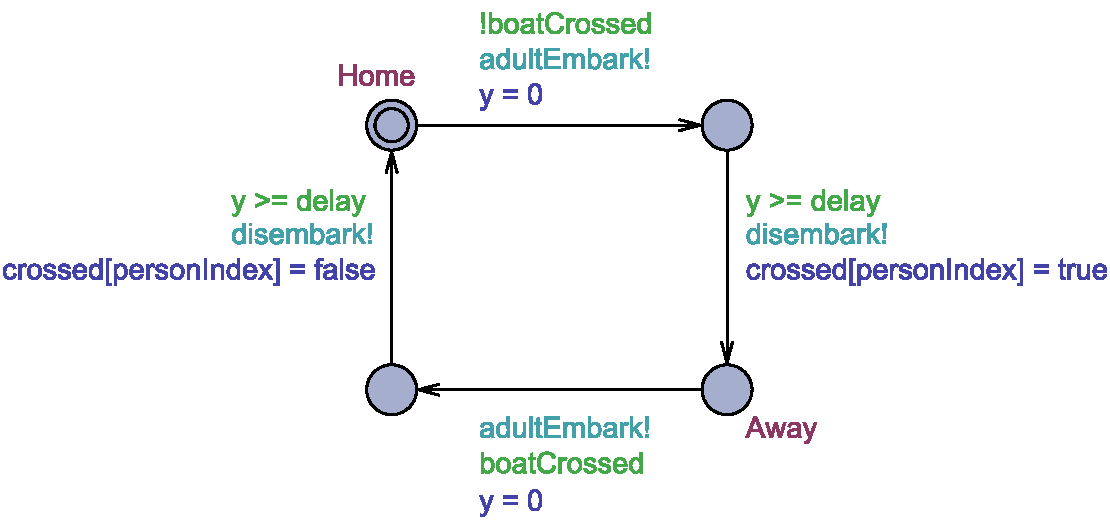
\includegraphics[width=\linewidth]{Adult.pdf}
\caption{Adult template}
\label{fig:adult}
\end{figure}

In order for an adult to be able to embark the boat from ``Home'', the guard \lstinline|boatCrossed| has to be false.  It uses the ``adultEmbark!'' channel to initiate the handshake with the boat in order to embark. When an adult disembarks the boat it initiates the handshake with ``disembark!'' , their boolean in \lstinline|crossed[personIndex]|, where ``personIndex'' is an index that is given when creating a new person, is changed to true. This indicates that the adult is ``Away''. 

An adult is able to embark the boat from ``Away'' if the \lstinline|boatCrossed| is true. When an adult disembarks the boat, their boolean is set to false. For now disregard the ``y'' variable. 

\begin{figure}[H]
\centering
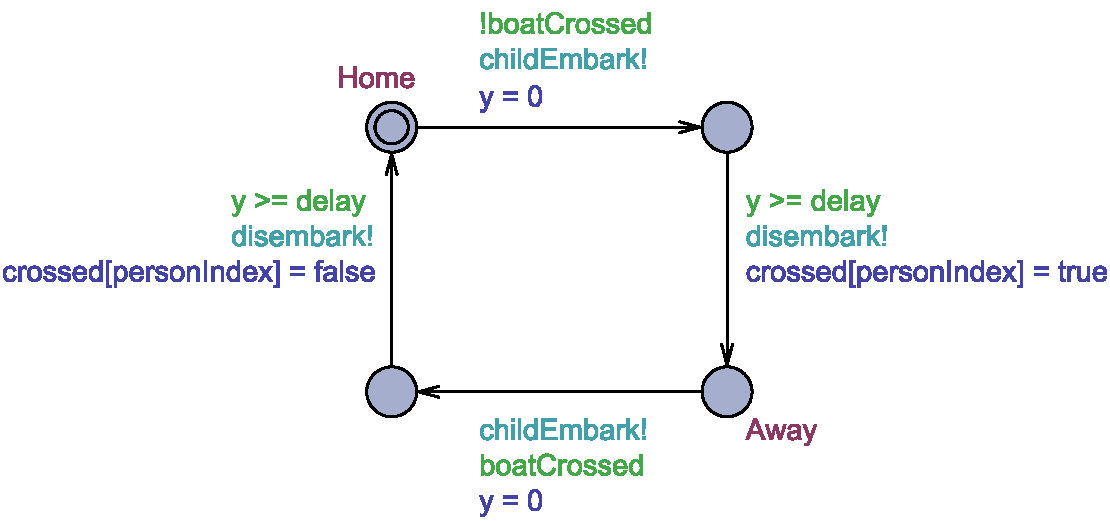
\includegraphics[width=\linewidth]{Child.pdf}
\caption{Child template}
\label{fig:child}
\end{figure}

The child template works exactly the same way as the adult template except it uses ``childEmbark!'' to initiate the handshake with the boat. The reason why is explained further down, in the explanation of the boat.

\begin{figure}[H]
\centering
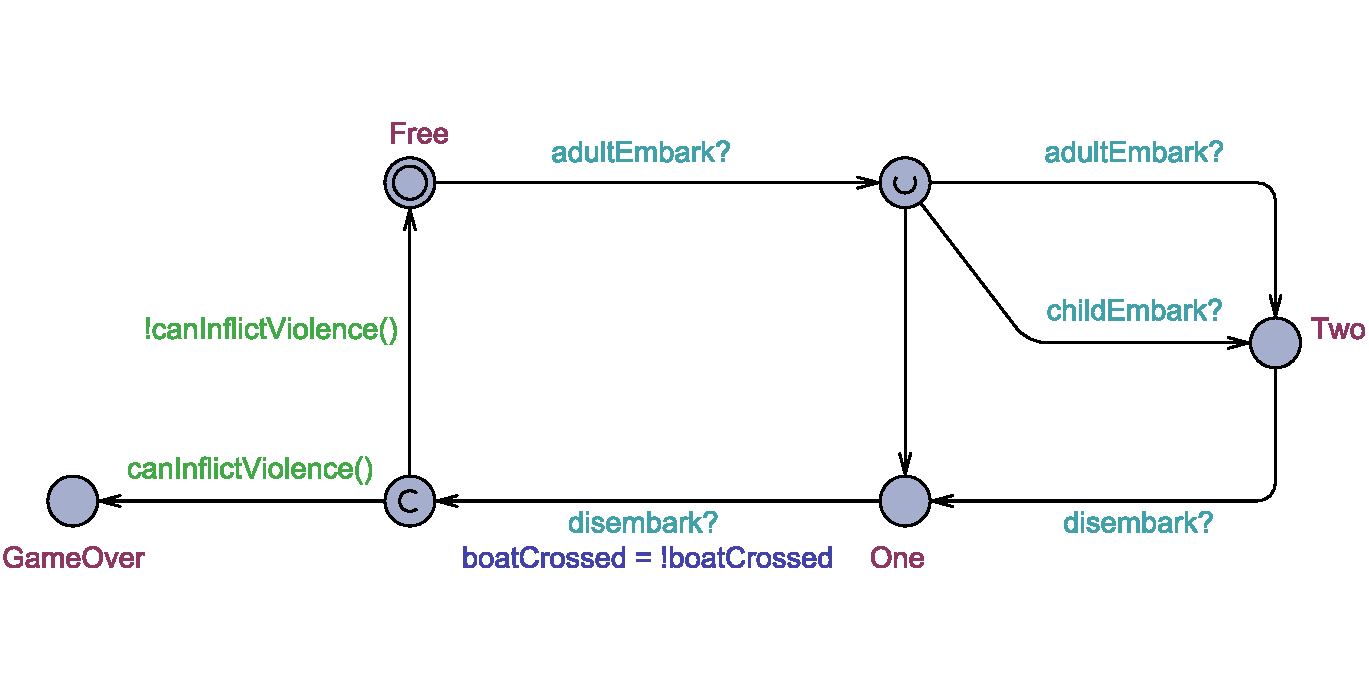
\includegraphics[width=\linewidth]{Boat.pdf}
\caption{Template for the boat}
\label{fig:boat}
\end{figure}

Figure \ref{fig:boat} shows the template for the boat. It has four marked locations, ``Free'', ``One'', ``Two'', and ``GameOver''. Free indicates that no one is on it. One means one person is on the boat and two means that two persons are on it. GameOver means the game is lost. 

Since two children, or a child and a thief are not allowed to cross the river at the same time, we decided to model the boat such that an adult has to embark the boat first before a child is allowed to embark, in order to save checks when the second person embarks in order to find out if the boat has two children or a child and a thief. After the adult has embarked the boat, either a child or an adult can embark. An adult is also able to cross the river alone. 

When the last person disembarks the boat a function called \lstinline|canInflictViolence()| is called. This function checks whether any person on either side can beat up any other person on the same side as themselves, in regards to the rules mentioned in the beginning. If \lstinline|canInflictViolence()| returns true then it goes to ``GameOver'' and the system is in a deadlock. If it returns false then the boat is ``Free'' and ready to be embarked.

The boat has two locations that are different from the others, it has an urgent and a committed location. After the first adult has embarked the boat, it is in an urgent location which means time must not pass while this location is part of the global state. 

This is where the ``y'' variable from both adult and child comes into play, the variable is used in order to keep track of time. Each person has a certain time they take the cross the river, and the boat sails with the speed of the slowest. In order to be sure that after an adult has embarked the boat, the time we have set it takes for him to cross the river does not pass, we have to ensure that the time does not pass until he either disembarks or another person embarks the boat.

After the last person has disembarked the system is in a committed stage, we chose this because we want to ensure that it is checked whether or not a person can inflict violence so that the game can continue.

All functions and variables are explained further down


\begin{lstlisting}[caption={Global declarations}]
// Place global declarations here.

clock time;
bool boatCrossed = false;
chan disembark, childEmbark, adultEmbark;

const int mom = 0;
const int dad = 1;
const int boy1 = 2;
const int boy2 = 3;
const int girl1 = 4;
const int girl2 = 5;
const int police1 = 6;
const int thief1 = 7;

const int boysCount = 3;
const int boys[boysCount] = { boy1, boy2 };

const int girlCount = 3;
const int girls[girlCount] = { girl1, girl2 };

const int policeCount = 2;
const int polices[policeCount] = { police1 };

const int thiefCount = 5;
const int thiefs[thiefCount] = { thief1 };

const int participants = boysCount + girlCount + policeCount + thiefCount + 2; // +2 for parents
bool crossed[participants]; // default array values are false

bool onTheSameSide(int p1, int p2)
{
    return crossed[p1] == crossed[p2];
}

bool boyOnSameSideAs(int personIndex)
{
    // if any boy is on the same side as the person, return true
    for (i : int[0, boysCount-1])
    {
        if (onTheSameSide(personIndex, boys[i]))
        {
            return true;
        }
    }
    return false;
}

bool girlOnSameSideAs(int personIndex)
{
    // if any girl is on the same side as the person, return true
    for (i : int[0, girlCount-1])
    {
        if (onTheSameSide(personIndex, girls[i]))
        {
            return true;
        }
    }
    return false;
}

bool policeOnTheSameSideAs(int personIndex)
{
    // if any dad is on the same side as the person, return true
    for (i : int[0, policeCount-1])
    {
        if (onTheSameSide(personIndex, polices[i]))
        {
            return true;
        }
    }
    return false;
}

bool canMomInflictViolence()
{
    return (boyOnSameSideAs(mom) && crossed[mom] != crossed[dad]);
}

bool canDadInflictViolence()
{
    return (girlOnSameSideAs(dad) && crossed[dad] != crossed[mom]);
}

bool canThiefInflictViolence()
{
    for (i : int [0, thiefCount-1])
    {
        int thiefIndex = thiefs[i];
        if (!policeOnTheSameSideAs(thiefIndex) && (crossed[thiefIndex] == crossed[mom] || crossed[thiefIndex] == crossed[dad] ||
           boyOnSameSideAs(thiefIndex) || girlOnSameSideAs(thiefIndex)))
        {
            return true;
        }
    }
    return false;
}

bool canInflictViolence()
{
    return canMomInflictViolence() || canDadInflictViolence() || canThiefInflictViolence();
}

bool allCrossed()
{
    for (i : int[0, participants-1])
    {
        if (!crossed[i])
        {
            return false;
        }
    }
    return true;
}
\end{lstlisting}

In order to create instances of \lstinline|Adult|s and \lstinline|Childs| we need to give them a unique index. The index is passed to the processes when they are declared as well as a constant amount of time they take to cross the river \lstinline|Boy1 = Child(boy1, fast)|.

All the unique indices are declared at lines 7-14 and the indices belonging to boys, girls, policemen, and thieves are put into their respective arrays at lines 16-27. So in order to add a boy/girl/policeman/thief to the system we only need to create a unique index $i$ such that $i \in [0 ... |participants|-1]$ which will correspond to their index in the \lstinline|crossed[ ]| array, then add the boy/girl/policeman/thief to their respective array, and remember to increment the count of that type of person. After that we of course also need to create the process for that person and them pass them their index.

If UPPAAL allowed us to get the size of an array passed as a parameter to a function then we could cut our code in half. We would not need to keep count of how many boys/girls/policemn/thieves we had, and we would only need one function to check whether a given person is on the same side as any type of person.

The \lstinline|allCrossed()| function checks whether all people in the game has crossed the river. This function is only used to query whether everyone crossed the river.

\section*{Conclusion}

With our UPPAAL model we can verify that it is possible to have everyone cross the river without anyone getting violent on each other. Trying to add just one boy/girl/thief leads to the game being unsolvable. If we add a policeman so we have two, then we can have as many boys/girls/thieves as we like.

We added time to our model. The childs/adults are then instantiated with the time they take to cross the river. Then with our global time variable, UPPAAL could see tell us the shortest time it takes for everyone to cross the river.

\end{document}